\documentclass[12pt]{book}

% Packages required by doxygen
\usepackage{fixltx2e}
\usepackage{calc}
\usepackage{doxygen}
\usepackage[export]{adjustbox} % also loads graphicx
\usepackage{graphicx}
\usepackage[utf8]{inputenc}
\usepackage{makeidx}
\usepackage{multicol}
\usepackage{multirow}
\PassOptionsToPackage{warn}{textcomp}
\usepackage{textcomp}
\usepackage[nointegrals]{wasysym}
\usepackage[table]{xcolor}

% Font selection
\usepackage[T1]{fontenc}
\usepackage[scaled=.90]{helvet}
\usepackage{courier}
\usepackage{amssymb}
\usepackage{sectsty}
\renewcommand{\familydefault}{\sfdefault}
\allsectionsfont{%
  \fontseries{bc}\selectfont%
  \color{darkgray}%
}
\renewcommand{\DoxyLabelFont}{%
  \fontseries{bc}\selectfont%
  \color{darkgray}%
}
\newcommand{\+}{\discretionary{\mbox{\scriptsize$\hookleftarrow$}}{}{}}

% Page & text layout
\usepackage{geometry}
\geometry{%
  a4paper,%
  top=2.5cm,%
  bottom=2.5cm,%
  left=2.5cm,%
  right=2.5cm%
}
\tolerance=750
\hfuzz=15pt
\hbadness=750
\setlength{\emergencystretch}{15pt}
\setlength{\parindent}{0cm}
\setlength{\parskip}{3ex plus 2ex minus 2ex}
\makeatletter
\renewcommand{\paragraph}{%
  \@startsection{paragraph}{4}{0ex}{-1.0ex}{1.0ex}{%
    \normalfont\normalsize\bfseries\SS@parafont%
  }%
}
\renewcommand{\subparagraph}{%
  \@startsection{subparagraph}{5}{0ex}{-1.0ex}{1.0ex}{%
    \normalfont\normalsize\bfseries\SS@subparafont%
  }%
}
\makeatother

% Headers & footers
\usepackage{fancyhdr}
\pagestyle{fancyplain}
\fancyhead[LE]{\fancyplain{}{\bfseries\thepage}}
\fancyhead[CE]{\fancyplain{}{}}
\fancyhead[RE]{\fancyplain{}{\bfseries\leftmark}}
\fancyhead[LO]{\fancyplain{}{\bfseries\rightmark}}
\fancyhead[CO]{\fancyplain{}{}}
\fancyhead[RO]{\fancyplain{}{\bfseries\thepage}}
\fancyfoot[LE]{\fancyplain{}{}}
\fancyfoot[CE]{\fancyplain{}{}}
\fancyfoot[RE]{\fancyplain{}{\bfseries\scriptsize Generated by Doxygen }}
\fancyfoot[LO]{\fancyplain{}{\bfseries\scriptsize Generated by Doxygen }}
\fancyfoot[CO]{\fancyplain{}{}}
\fancyfoot[RO]{\fancyplain{}{}}
\renewcommand{\footrulewidth}{0.4pt}
\renewcommand{\chaptermark}[1]{%
  \markboth{#1}{}%
}
\renewcommand{\sectionmark}[1]{%
  \markright{\thesection\ #1}%
}

% Indices & bibliography
\usepackage{natbib}
\usepackage[titles]{tocloft}
\setcounter{tocdepth}{3}
\setcounter{secnumdepth}{5}
\makeindex

% Hyperlinks (required, but should be loaded last)
\usepackage{ifpdf}
\ifpdf
  \usepackage[pdftex,pagebackref=true]{hyperref}
\else
  \usepackage[ps2pdf,pagebackref=true]{hyperref}
\fi
\hypersetup{%
  colorlinks=true,%
  linkcolor=blue,%
  citecolor=blue,%
  unicode%
}

% Custom commands
\newcommand{\clearemptydoublepage}{%
  \newpage{\pagestyle{empty}\cleardoublepage}%
}

\usepackage{caption}
\captionsetup{labelsep=space,justification=centering,font={bf},singlelinecheck=off,skip=4pt,position=top}

%===== C O N T E N T S =====

\begin{document}

% Titlepage & ToC
\hypersetup{pageanchor=false,
             bookmarksnumbered=true,
             pdfencoding=unicode
            }
\pagenumbering{alph}
\begin{titlepage}
\vspace*{7cm}
\begin{center}%
{\LARGE \textbf{Project 1: Event Planner}}\\
{\Large \textit{Team 3}}\\
\vspace*{1cm}
%{\large Generated by Doxygen 1.8.14}\\
\end{center}
\end{titlepage}
\pagenumbering{roman}
\tableofcontents
\pagenumbering{arabic}
\hypersetup{pageanchor=true}

%--- Begin generated contents ---
\chapter{Class Index}
\section{Class List}
Here are the classes, structs, unions and interfaces with brief descriptions\+:\begin{DoxyCompactList}
\item\contentsline{section}{\mbox{\hyperlink{class_events}{Events}} }{\pageref{class_events}}{}
\item\contentsline{section}{\mbox{\hyperlink{class_interface}{Interface}} }{\pageref{class_interface}}{}
\item\contentsline{section}{\mbox{\hyperlink{class_i_o}{IO}} \\*A header file for Input/\+Output (\mbox{\hyperlink{class_i_o}{IO}}) class }{\pageref{class_i_o}}{}
\item\contentsline{section}{\mbox{\hyperlink{class_log}{Log}} \\*A header file \mbox{\hyperlink{class_log}{Log}} class }{\pageref{class_log}}{}
\item\contentsline{section}{\mbox{\hyperlink{class_interface_1_1_menu}{Interface\+::\+Menu}} }{\pageref{class_interface_1_1_menu}}{}
\end{DoxyCompactList}

\chapter{File Index}
\section{File List}
Here is a list of all documented files with brief descriptions\+:\begin{DoxyCompactList}
\item\contentsline{section}{{\bfseries events.\+h} }{\pageref{events_8h}}{}
\item\contentsline{section}{\hyperlink{events_8hpp}{events.\+hpp} }{\pageref{events_8hpp}}{}
\item\contentsline{section}{{\bfseries interface.\+h} }{\pageref{interface_8h}}{}
\item\contentsline{section}{\hyperlink{interface_8hpp}{interface.\+hpp} }{\pageref{interface_8hpp}}{}
\item\contentsline{section}{{\bfseries io.\+h} }{\pageref{io_8h}}{}
\item\contentsline{section}{\hyperlink{io_8hpp}{io.\+hpp} }{\pageref{io_8hpp}}{}
\item\contentsline{section}{{\bfseries log.\+h} }{\pageref{log_8h}}{}
\item\contentsline{section}{\hyperlink{log_8hpp}{log.\+hpp} }{\pageref{log_8hpp}}{}
\item\contentsline{section}{\hyperlink{main_8cpp}{main.\+cpp} \\*Driver for project }{\pageref{main_8cpp}}{}
\end{DoxyCompactList}

\chapter{Class Documentation}
\hypertarget{class_events}{}\section{Events Class Reference}
\label{class_events}\index{Events@{Events}}
\subsection*{Static Public Member Functions}
\begin{DoxyCompactItemize}
\item 
static void \mbox{\hyperlink{class_events_a2fdb7c40bf64aa2e23d3d92dc7ab4d35}{user\+Mode}} ()
\item 
static void \mbox{\hyperlink{class_events_a2217e32868e367ec8d432ce9db2b450e}{admin\+Mode}} ()
\end{DoxyCompactItemize}


\subsection{Member Function Documentation}
\mbox{\Hypertarget{class_events_a2217e32868e367ec8d432ce9db2b450e}\label{class_events_a2217e32868e367ec8d432ce9db2b450e}} 
\index{Events@{Events}!admin\+Mode@{admin\+Mode}}
\index{admin\+Mode@{admin\+Mode}!Events@{Events}}
\subsubsection{\texorpdfstring{admin\+Mode()}{adminMode()}}
{\footnotesize\ttfamily void Events\+::admin\+Mode (\begin{DoxyParamCaption}{ }\end{DoxyParamCaption})\hspace{0.3cm}{\ttfamily [static]}}

\begin{DoxyPrecond}{Precondition}
None 
\end{DoxyPrecond}
\begin{DoxyPostcond}{Postcondition}
Start Admin Mode 
\end{DoxyPostcond}
\begin{DoxyReturn}{Returns}
None 
\end{DoxyReturn}
\mbox{\Hypertarget{class_events_a2fdb7c40bf64aa2e23d3d92dc7ab4d35}\label{class_events_a2fdb7c40bf64aa2e23d3d92dc7ab4d35}} 
\index{Events@{Events}!user\+Mode@{user\+Mode}}
\index{user\+Mode@{user\+Mode}!Events@{Events}}
\subsubsection{\texorpdfstring{user\+Mode()}{userMode()}}
{\footnotesize\ttfamily void Events\+::user\+Mode (\begin{DoxyParamCaption}{ }\end{DoxyParamCaption})\hspace{0.3cm}{\ttfamily [static]}}

\begin{DoxyPrecond}{Precondition}
None 
\end{DoxyPrecond}
\begin{DoxyPostcond}{Postcondition}
Start User Mode 
\end{DoxyPostcond}
\begin{DoxyReturn}{Returns}
None 
\end{DoxyReturn}


The documentation for this class was generated from the following files\+:\begin{DoxyCompactItemize}
\item 
events.\+h\item 
\mbox{\hyperlink{events_8hpp}{events.\+hpp}}\end{DoxyCompactItemize}

\hypertarget{class_interface}{}\section{Interface Class Reference}
\label{class_interface}\index{Interface@{Interface}}
\subsection*{Classes}
\begin{DoxyCompactItemize}
\item 
class \mbox{\hyperlink{class_interface_1_1_menu}{Menu}}
\end{DoxyCompactItemize}
\subsection*{Public Member Functions}
\begin{DoxyCompactItemize}
\item 
\mbox{\hyperlink{class_interface_a4406d74c75bdfe150bf72be1f1cda8b1}{Interface}} ()
\item 
\mbox{\hyperlink{class_interface_a19179888f29f18f1be54a3dfe98f68c0}{$\sim$\+Interface}} ()
\end{DoxyCompactItemize}
\subsection*{Static Public Member Functions}
\begin{DoxyCompactItemize}
\item 
static void \mbox{\hyperlink{class_interface_af92bb2aeecc6a19095af23fa78b49451}{clear\+Screen}} ()
\item 
static std\+::string \mbox{\hyperlink{class_interface_aa5c0539404373d488986f030f7a84a6f}{get\+Input}} (const char $\ast$message)
\item 
static void \mbox{\hyperlink{class_interface_ab235ba2f0184e3fbfd5d5a64d5eb85ef}{Wait}} (std\+::string wait\+\_\+string)
\item 
static void \mbox{\hyperlink{class_interface_a2e002e61dc11cf4a1bd9c039704194df}{toggle\+Time\+Format}} ()
\end{DoxyCompactItemize}


\subsection{Constructor \& Destructor Documentation}
\mbox{\Hypertarget{class_interface_a4406d74c75bdfe150bf72be1f1cda8b1}\label{class_interface_a4406d74c75bdfe150bf72be1f1cda8b1}} 
\index{Interface@{Interface}!Interface@{Interface}}
\index{Interface@{Interface}!Interface@{Interface}}
\subsubsection{\texorpdfstring{Interface()}{Interface()}}
{\footnotesize\ttfamily Interface\+::\+Interface (\begin{DoxyParamCaption}{ }\end{DoxyParamCaption})}

\begin{DoxyPrecond}{Precondition}
None 
\end{DoxyPrecond}
\begin{DoxyPostcond}{Postcondition}
Constructor 
\end{DoxyPostcond}
\mbox{\Hypertarget{class_interface_a19179888f29f18f1be54a3dfe98f68c0}\label{class_interface_a19179888f29f18f1be54a3dfe98f68c0}} 
\index{Interface@{Interface}!````~Interface@{$\sim$\+Interface}}
\index{````~Interface@{$\sim$\+Interface}!Interface@{Interface}}
\subsubsection{\texorpdfstring{$\sim$\+Interface()}{~Interface()}}
{\footnotesize\ttfamily Interface\+::$\sim$\+Interface (\begin{DoxyParamCaption}{ }\end{DoxyParamCaption})}

\begin{DoxyPrecond}{Precondition}
None 
\end{DoxyPrecond}
\begin{DoxyPostcond}{Postcondition}
Destructor 
\end{DoxyPostcond}


\subsection{Member Function Documentation}
\mbox{\Hypertarget{class_interface_af92bb2aeecc6a19095af23fa78b49451}\label{class_interface_af92bb2aeecc6a19095af23fa78b49451}} 
\index{Interface@{Interface}!clear\+Screen@{clear\+Screen}}
\index{clear\+Screen@{clear\+Screen}!Interface@{Interface}}
\subsubsection{\texorpdfstring{clear\+Screen()}{clearScreen()}}
{\footnotesize\ttfamily void Interface\+::clear\+Screen (\begin{DoxyParamCaption}{ }\end{DoxyParamCaption})\hspace{0.3cm}{\ttfamily [static]}}

\begin{DoxyPrecond}{Precondition}
None 
\end{DoxyPrecond}
\begin{DoxyPostcond}{Postcondition}
Clears terminal 
\end{DoxyPostcond}
\begin{DoxyReturn}{Returns}
None 
\end{DoxyReturn}
\mbox{\Hypertarget{class_interface_aa5c0539404373d488986f030f7a84a6f}\label{class_interface_aa5c0539404373d488986f030f7a84a6f}} 
\index{Interface@{Interface}!get\+Input@{get\+Input}}
\index{get\+Input@{get\+Input}!Interface@{Interface}}
\subsubsection{\texorpdfstring{get\+Input()}{getInput()}}
{\footnotesize\ttfamily std\+::string Interface\+::get\+Input (\begin{DoxyParamCaption}\item[{const char $\ast$}]{message }\end{DoxyParamCaption})\hspace{0.3cm}{\ttfamily [static]}}

\begin{DoxyPrecond}{Precondition}
message is the input request message string presented to the user 
\end{DoxyPrecond}
\begin{DoxyPostcond}{Postcondition}
requests user input 
\end{DoxyPostcond}
\begin{DoxyReturn}{Returns}
Returns the user\textquotesingle{}s given input 
\end{DoxyReturn}
\mbox{\Hypertarget{class_interface_a2e002e61dc11cf4a1bd9c039704194df}\label{class_interface_a2e002e61dc11cf4a1bd9c039704194df}} 
\index{Interface@{Interface}!toggle\+Time\+Format@{toggle\+Time\+Format}}
\index{toggle\+Time\+Format@{toggle\+Time\+Format}!Interface@{Interface}}
\subsubsection{\texorpdfstring{toggle\+Time\+Format()}{toggleTimeFormat()}}
{\footnotesize\ttfamily void Interface\+::toggle\+Time\+Format (\begin{DoxyParamCaption}{ }\end{DoxyParamCaption})\hspace{0.3cm}{\ttfamily [static]}}

\begin{DoxyPrecond}{Precondition}
None 
\end{DoxyPrecond}
\begin{DoxyPostcond}{Postcondition}
Toggles the time format between 12-\/hour and 24-\/hour formats 
\end{DoxyPostcond}
\begin{DoxyReturn}{Returns}
None 
\end{DoxyReturn}
\mbox{\Hypertarget{class_interface_ab235ba2f0184e3fbfd5d5a64d5eb85ef}\label{class_interface_ab235ba2f0184e3fbfd5d5a64d5eb85ef}} 
\index{Interface@{Interface}!Wait@{Wait}}
\index{Wait@{Wait}!Interface@{Interface}}
\subsubsection{\texorpdfstring{Wait()}{Wait()}}
{\footnotesize\ttfamily void Interface\+::\+Wait (\begin{DoxyParamCaption}\item[{std\+::string}]{wait\+\_\+string }\end{DoxyParamCaption})\hspace{0.3cm}{\ttfamily [static]}}

\begin{DoxyPrecond}{Precondition}
wait\+\_\+string is a message shown to the user while waiting 
\end{DoxyPrecond}
\begin{DoxyPostcond}{Postcondition}
Waits for the user to press enter 
\end{DoxyPostcond}
\begin{DoxyReturn}{Returns}
None 
\end{DoxyReturn}


The documentation for this class was generated from the following files\+:\begin{DoxyCompactItemize}
\item 
interface.\+h\item 
\mbox{\hyperlink{interface_8hpp}{interface.\+hpp}}\end{DoxyCompactItemize}

\hypertarget{class_i_o}{}\section{IO Class Reference}
\label{class_i_o}\index{IO@{IO}}


A header file for Input/\+Output (\mbox{\hyperlink{class_i_o}{IO}}) class.  




{\ttfamily \#include $<$io.\+h$>$}

\subsection*{Public Member Functions}
\begin{DoxyCompactItemize}
\item 
\mbox{\hyperlink{class_i_o_a98e1371822dc63d6b25c4153efd1bbf3}{IO}} (const std\+::string file\+Name)
\item 
\mbox{\hyperlink{class_i_o_a44861ff225d351615179f0f24cb8d7f6}{$\sim$\+IO}} ()
\item 
void \mbox{\hyperlink{class_i_o_aa3537c0737038acdc6c2963138bfabdf}{add\+Entry}} (std\+::string store)
\item 
std\+::string \mbox{\hyperlink{class_i_o_a3829dc8ad91e1f2d560be799b6d9b04d}{retrieve\+Element}} (int ID, std\+::string element\+Name)
\item 
void \mbox{\hyperlink{class_i_o_a11fdb7d4afa830fa1441fbf566f73432}{update\+Element}} (int ID, std\+::string element\+Name, void $\ast$value)
\item 
void \mbox{\hyperlink{class_i_o_a48e9febfbb2c6c3e01b467fd030c2529}{display\+Entries}} ()
\item 
std\+::string \mbox{\hyperlink{class_i_o_ad78c42847c70915fe94bddd25f716859}{time\+Formatter}} (std\+::string slot)
\end{DoxyCompactItemize}
\subsection*{Public Attributes}
\begin{DoxyCompactItemize}
\item 
\mbox{\Hypertarget{class_i_o_a4e344c74454e6609b817e3fdb3fcddf3}\label{class_i_o_a4e344c74454e6609b817e3fdb3fcddf3}} 
int {\bfseries size}
\end{DoxyCompactItemize}
\subsection*{Static Public Attributes}
\begin{DoxyCompactItemize}
\item 
\mbox{\Hypertarget{class_i_o_a04cf024687a6a86007db5ecfcab69e5c}\label{class_i_o_a04cf024687a6a86007db5ecfcab69e5c}} 
static bool {\bfseries time\+Format} = false
\end{DoxyCompactItemize}


\subsection{Detailed Description}
A header file for Input/\+Output (\mbox{\hyperlink{class_i_o}{IO}}) class. 

\begin{DoxyAuthor}{Author}
Team 3 
\end{DoxyAuthor}
\begin{DoxyDate}{Date}

\end{DoxyDate}


\subsection{Constructor \& Destructor Documentation}
\mbox{\Hypertarget{class_i_o_a98e1371822dc63d6b25c4153efd1bbf3}\label{class_i_o_a98e1371822dc63d6b25c4153efd1bbf3}} 
\index{IO@{IO}!IO@{IO}}
\index{IO@{IO}!IO@{IO}}
\subsubsection{\texorpdfstring{I\+O()}{IO()}}
{\footnotesize\ttfamily I\+O\+::\+IO (\begin{DoxyParamCaption}\item[{const std\+::string}]{file\+Name }\end{DoxyParamCaption})}

\begin{DoxyPrecond}{Precondition}
None 
\end{DoxyPrecond}
\begin{DoxyPostcond}{Postcondition}
A file is opened with given name. It is created if it does not exist yet 
\end{DoxyPostcond}
\mbox{\Hypertarget{class_i_o_a44861ff225d351615179f0f24cb8d7f6}\label{class_i_o_a44861ff225d351615179f0f24cb8d7f6}} 
\index{IO@{IO}!````~IO@{$\sim$\+IO}}
\index{````~IO@{$\sim$\+IO}!IO@{IO}}
\subsubsection{\texorpdfstring{$\sim$\+I\+O()}{~IO()}}
{\footnotesize\ttfamily I\+O\+::$\sim$\+IO (\begin{DoxyParamCaption}{ }\end{DoxyParamCaption})}

\begin{DoxyPrecond}{Precondition}
None 
\end{DoxyPrecond}
\begin{DoxyPostcond}{Postcondition}
A file is closed with given name 
\end{DoxyPostcond}


\subsection{Member Function Documentation}
\mbox{\Hypertarget{class_i_o_aa3537c0737038acdc6c2963138bfabdf}\label{class_i_o_aa3537c0737038acdc6c2963138bfabdf}} 
\index{IO@{IO}!add\+Entry@{add\+Entry}}
\index{add\+Entry@{add\+Entry}!IO@{IO}}
\subsubsection{\texorpdfstring{add\+Entry()}{addEntry()}}
{\footnotesize\ttfamily void I\+O\+::add\+Entry (\begin{DoxyParamCaption}\item[{std\+::string}]{store }\end{DoxyParamCaption})}

\begin{DoxyPrecond}{Precondition}
None 
\end{DoxyPrecond}
\begin{DoxyPostcond}{Postcondition}
Adds new event to file 
\end{DoxyPostcond}
\begin{DoxyReturn}{Returns}
None 
\end{DoxyReturn}
\mbox{\Hypertarget{class_i_o_a48e9febfbb2c6c3e01b467fd030c2529}\label{class_i_o_a48e9febfbb2c6c3e01b467fd030c2529}} 
\index{IO@{IO}!display\+Entries@{display\+Entries}}
\index{display\+Entries@{display\+Entries}!IO@{IO}}
\subsubsection{\texorpdfstring{display\+Entries()}{displayEntries()}}
{\footnotesize\ttfamily void I\+O\+::display\+Entries (\begin{DoxyParamCaption}{ }\end{DoxyParamCaption})}

\begin{DoxyPrecond}{Precondition}
None 
\end{DoxyPrecond}
\begin{DoxyPostcond}{Postcondition}
Displays all elements in file, one at a time 
\end{DoxyPostcond}
\begin{DoxyReturn}{Returns}
None 
\end{DoxyReturn}
\mbox{\Hypertarget{class_i_o_a3829dc8ad91e1f2d560be799b6d9b04d}\label{class_i_o_a3829dc8ad91e1f2d560be799b6d9b04d}} 
\index{IO@{IO}!retrieve\+Element@{retrieve\+Element}}
\index{retrieve\+Element@{retrieve\+Element}!IO@{IO}}
\subsubsection{\texorpdfstring{retrieve\+Element()}{retrieveElement()}}
{\footnotesize\ttfamily std\+::string I\+O\+::retrieve\+Element (\begin{DoxyParamCaption}\item[{int}]{ID,  }\item[{std\+::string}]{element\+Name }\end{DoxyParamCaption})}

\begin{DoxyPrecond}{Precondition}
ID is the event\textquotesingle{}s unique identifier. element\+Name is the name of the element to retrieve 
\end{DoxyPrecond}
\begin{DoxyPostcond}{Postcondition}
Retrieves some event\textquotesingle{}s specific element value from the events file 
\end{DoxyPostcond}
\begin{DoxyReturn}{Returns}
Returns event\textquotesingle{}s specific element (string or int) 
\end{DoxyReturn}
\mbox{\Hypertarget{class_i_o_ad78c42847c70915fe94bddd25f716859}\label{class_i_o_ad78c42847c70915fe94bddd25f716859}} 
\index{IO@{IO}!time\+Formatter@{time\+Formatter}}
\index{time\+Formatter@{time\+Formatter}!IO@{IO}}
\subsubsection{\texorpdfstring{time\+Formatter()}{timeFormatter()}}
{\footnotesize\ttfamily std\+::string I\+O\+::time\+Formatter (\begin{DoxyParamCaption}\item[{std\+::string}]{slot }\end{DoxyParamCaption})}

\begin{DoxyPrecond}{Precondition}
slot has the time value that needs to be formatted 
\end{DoxyPrecond}
\begin{DoxyPostcond}{Postcondition}
Formats time between 12-\/hour format and 24-\/hour format 
\end{DoxyPostcond}
\begin{DoxyReturn}{Returns}
String with slot in new time format 
\end{DoxyReturn}
\mbox{\Hypertarget{class_i_o_a11fdb7d4afa830fa1441fbf566f73432}\label{class_i_o_a11fdb7d4afa830fa1441fbf566f73432}} 
\index{IO@{IO}!update\+Element@{update\+Element}}
\index{update\+Element@{update\+Element}!IO@{IO}}
\subsubsection{\texorpdfstring{update\+Element()}{updateElement()}}
{\footnotesize\ttfamily void I\+O\+::update\+Element (\begin{DoxyParamCaption}\item[{int}]{ID,  }\item[{std\+::string}]{element\+Name,  }\item[{void $\ast$}]{value }\end{DoxyParamCaption})}

\begin{DoxyPrecond}{Precondition}
ID is the event\textquotesingle{}s unique identifier. element\+Name is the name of the element to update, value is the element\textquotesingle{}s new value 
\end{DoxyPrecond}
\begin{DoxyPostcond}{Postcondition}
Updates some event\textquotesingle{}s specific element 
\end{DoxyPostcond}
\begin{DoxyReturn}{Returns}
None 
\end{DoxyReturn}


The documentation for this class was generated from the following files\+:\begin{DoxyCompactItemize}
\item 
io.\+h\item 
\mbox{\hyperlink{io_8hpp}{io.\+hpp}}\end{DoxyCompactItemize}

\hypertarget{class_log}{}\section{Log Class Reference}
\label{class_log}\index{Log@{Log}}


A header file \mbox{\hyperlink{class_log}{Log}} class.  




{\ttfamily \#include $<$log.\+h$>$}

\subsection*{Public Member Functions}
\begin{DoxyCompactItemize}
\item 
\mbox{\hyperlink{class_log_af6071a60aa52b6c1b511f99b4bc1b8fe}{Log}} ()
\item 
\mbox{\hyperlink{class_log_a0fbfda88fbee5027c89f6eb121059360}{$\sim$\+Log}} ()
\item 
void \mbox{\hyperlink{class_log_a1ccb79c34552336f3bd399b7c9b035d7}{add\+Entry}} (std\+::string error\+\_\+type, std\+::string function\+\_\+responsible)
\end{DoxyCompactItemize}


\subsection{Detailed Description}
A header file \mbox{\hyperlink{class_log}{Log}} class. 

\begin{DoxyAuthor}{Author}
Team 3 
\end{DoxyAuthor}
\begin{DoxyDate}{Date}

\end{DoxyDate}


\subsection{Constructor \& Destructor Documentation}
\mbox{\Hypertarget{class_log_af6071a60aa52b6c1b511f99b4bc1b8fe}\label{class_log_af6071a60aa52b6c1b511f99b4bc1b8fe}} 
\index{Log@{Log}!Log@{Log}}
\index{Log@{Log}!Log@{Log}}
\subsubsection{\texorpdfstring{Log()}{Log()}}
{\footnotesize\ttfamily Log\+::\+Log (\begin{DoxyParamCaption}{ }\end{DoxyParamCaption})}

\begin{DoxyPrecond}{Precondition}
None 
\end{DoxyPrecond}
\begin{DoxyPostcond}{Postcondition}
A file is opened with given name. It is created if it does not exist yet 
\end{DoxyPostcond}
\mbox{\Hypertarget{class_log_a0fbfda88fbee5027c89f6eb121059360}\label{class_log_a0fbfda88fbee5027c89f6eb121059360}} 
\index{Log@{Log}!````~Log@{$\sim$\+Log}}
\index{````~Log@{$\sim$\+Log}!Log@{Log}}
\subsubsection{\texorpdfstring{$\sim$\+Log()}{~Log()}}
{\footnotesize\ttfamily Log\+::$\sim$\+Log (\begin{DoxyParamCaption}{ }\end{DoxyParamCaption})}

\begin{DoxyPrecond}{Precondition}
None 
\end{DoxyPrecond}
\begin{DoxyPostcond}{Postcondition}
A file is closed with given name 
\end{DoxyPostcond}


\subsection{Member Function Documentation}
\mbox{\Hypertarget{class_log_a1ccb79c34552336f3bd399b7c9b035d7}\label{class_log_a1ccb79c34552336f3bd399b7c9b035d7}} 
\index{Log@{Log}!add\+Entry@{add\+Entry}}
\index{add\+Entry@{add\+Entry}!Log@{Log}}
\subsubsection{\texorpdfstring{add\+Entry()}{addEntry()}}
{\footnotesize\ttfamily void Log\+::add\+Entry (\begin{DoxyParamCaption}\item[{std\+::string}]{error\+\_\+type,  }\item[{std\+::string}]{function\+\_\+responsible }\end{DoxyParamCaption})}

\begin{DoxyPrecond}{Precondition}
time\+Ndate refers to the specific time and date the error occurred, error\+\_\+type specifies the type of error encoutered, function\+\_\+responsible specifies where the error occurred in the code 
\end{DoxyPrecond}
\begin{DoxyPostcond}{Postcondition}
Keeps log file of encountered errors in the running program. Shows error message to user 
\end{DoxyPostcond}
\begin{DoxyReturn}{Returns}
None 
\end{DoxyReturn}


The documentation for this class was generated from the following files\+:\begin{DoxyCompactItemize}
\item 
log.\+h\item 
\mbox{\hyperlink{log_8hpp}{log.\+hpp}}\end{DoxyCompactItemize}

\hypertarget{class_interface_1_1_menu}{}\section{Interface\+:\+:Menu Class Reference}
\label{class_interface_1_1_menu}\index{Interface\+::\+Menu@{Interface\+::\+Menu}}
\subsection*{Public Member Functions}
\begin{DoxyCompactItemize}
\item 
\mbox{\hyperlink{class_interface_1_1_menu_ad9d0ce403f0ad96df24bcde018030650}{Menu}} (const std\+::vector$<$ std\+::pair$<$ std\+::string, void($\ast$)()$>$$>$ \&options)
\item 
void \mbox{\hyperlink{class_interface_1_1_menu_ac6e7791ff9ffb233d07e05653a4f5bb2}{Loop}} ()
\item 
void \mbox{\hyperlink{class_interface_1_1_menu_ac9c262f57118f3b3043bed327f195c00}{Header}} ()
\end{DoxyCompactItemize}


\subsection{Constructor \& Destructor Documentation}
\mbox{\Hypertarget{class_interface_1_1_menu_ad9d0ce403f0ad96df24bcde018030650}\label{class_interface_1_1_menu_ad9d0ce403f0ad96df24bcde018030650}} 
\index{Interface\+::\+Menu@{Interface\+::\+Menu}!Menu@{Menu}}
\index{Menu@{Menu}!Interface\+::\+Menu@{Interface\+::\+Menu}}
\subsubsection{\texorpdfstring{Menu()}{Menu()}}
{\footnotesize\ttfamily Interface\+::\+Menu\+::\+Menu (\begin{DoxyParamCaption}\item[{const std\+::vector$<$ std\+::pair$<$ std\+::string, void($\ast$)()$>$$>$ \&}]{options }\end{DoxyParamCaption})}

\begin{DoxyPrecond}{Precondition}
options is a vector of pairs, where each pair is composed of a string (referring to a menu option, and a pointer to the corresponding callback function 
\end{DoxyPrecond}
\begin{DoxyPostcond}{Postcondition}
Constructor for \mbox{\hyperlink{class_interface_1_1_menu}{Menu}} class object 
\end{DoxyPostcond}


\subsection{Member Function Documentation}
\mbox{\Hypertarget{class_interface_1_1_menu_ac9c262f57118f3b3043bed327f195c00}\label{class_interface_1_1_menu_ac9c262f57118f3b3043bed327f195c00}} 
\index{Interface\+::\+Menu@{Interface\+::\+Menu}!Header@{Header}}
\index{Header@{Header}!Interface\+::\+Menu@{Interface\+::\+Menu}}
\subsubsection{\texorpdfstring{Header()}{Header()}}
{\footnotesize\ttfamily void Interface\+::\+Menu\+::\+Header (\begin{DoxyParamCaption}{ }\end{DoxyParamCaption})}

\begin{DoxyPrecond}{Precondition}
None 
\end{DoxyPrecond}
\begin{DoxyPostcond}{Postcondition}
Draws a header for a menu 
\end{DoxyPostcond}
\begin{DoxyReturn}{Returns}
None 
\end{DoxyReturn}
\mbox{\Hypertarget{class_interface_1_1_menu_ac6e7791ff9ffb233d07e05653a4f5bb2}\label{class_interface_1_1_menu_ac6e7791ff9ffb233d07e05653a4f5bb2}} 
\index{Interface\+::\+Menu@{Interface\+::\+Menu}!Loop@{Loop}}
\index{Loop@{Loop}!Interface\+::\+Menu@{Interface\+::\+Menu}}
\subsubsection{\texorpdfstring{Loop()}{Loop()}}
{\footnotesize\ttfamily void Interface\+::\+Menu\+::\+Loop (\begin{DoxyParamCaption}{ }\end{DoxyParamCaption})}

\begin{DoxyPrecond}{Precondition}
None 
\end{DoxyPrecond}
\begin{DoxyPostcond}{Postcondition}
A menu loop 
\end{DoxyPostcond}
\begin{DoxyReturn}{Returns}
None 
\end{DoxyReturn}


The documentation for this class was generated from the following files\+:\begin{DoxyCompactItemize}
\item 
interface.\+h\item 
\mbox{\hyperlink{interface_8hpp}{interface.\+hpp}}\end{DoxyCompactItemize}

\chapter{File Documentation}
\hypertarget{events_8hpp}{}\section{events.\+hpp File Reference}
\label{events_8hpp}\index{events.\+hpp@{events.\+hpp}}


\subsection{Detailed Description}
\begin{DoxyAuthor}{Author}
Team 3 
\end{DoxyAuthor}
\begin{DoxyDate}{Date}

\end{DoxyDate}

\hypertarget{interface_8hpp}{}\section{interface.\+hpp File Reference}
\label{interface_8hpp}\index{interface.\+hpp@{interface.\+hpp}}


\subsection{Detailed Description}
\begin{DoxyAuthor}{Author}
Team 3 
\end{DoxyAuthor}
\begin{DoxyDate}{Date}

\end{DoxyDate}

\hypertarget{io_8hpp}{}\section{io.\+hpp File Reference}
\label{io_8hpp}\index{io.\+hpp@{io.\+hpp}}
This graph shows which files directly or indirectly include this file\+:
\nopagebreak
\begin{figure}[H]
\begin{center}
\leavevmode
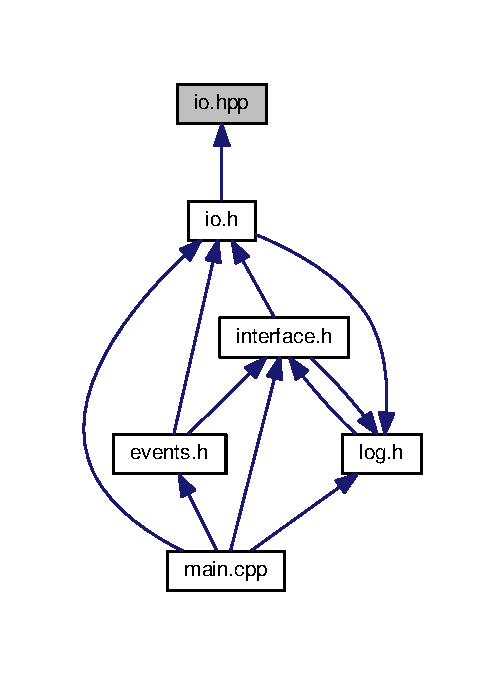
\includegraphics[width=242pt]{io_8hpp__dep__incl}
\end{center}
\end{figure}


\subsection{Detailed Description}
\begin{DoxyAuthor}{Author}
Team 3 
\end{DoxyAuthor}
\begin{DoxyDate}{Date}

\end{DoxyDate}

\hypertarget{log_8hpp}{}\section{log.\+hpp File Reference}
\label{log_8hpp}\index{log.\+hpp@{log.\+hpp}}
This graph shows which files directly or indirectly include this file\+:\nopagebreak
\begin{figure}[H]
\begin{center}
\leavevmode
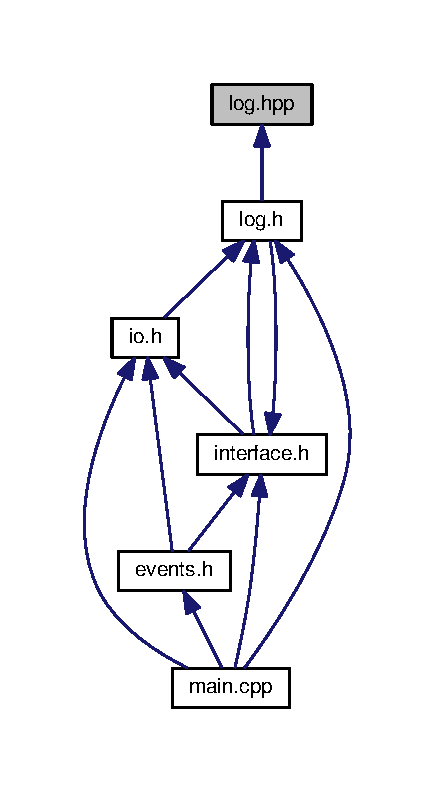
\includegraphics[width=209pt]{log_8hpp__dep__incl}
\end{center}
\end{figure}


\subsection{Detailed Description}
\begin{DoxyAuthor}{Author}
Team 3 
\end{DoxyAuthor}
\begin{DoxyDate}{Date}

\end{DoxyDate}

\hypertarget{main_8cpp}{}\section{main.\+cpp File Reference}
\label{main_8cpp}\index{main.\+cpp@{main.\+cpp}}


driver for project  


{\ttfamily \#include $<$iostream$>$}\\*
{\ttfamily \#include \char`\"{}interface.\+h\char`\"{}}\\*
{\ttfamily \#include \char`\"{}io.\+h\char`\"{}}\\*
{\ttfamily \#include \char`\"{}log.\+h\char`\"{}}\\*
{\ttfamily \#include \char`\"{}events.\+h\char`\"{}}\\*
Include dependency graph for main.\+cpp\+:\nopagebreak
\begin{figure}[H]
\begin{center}
\leavevmode
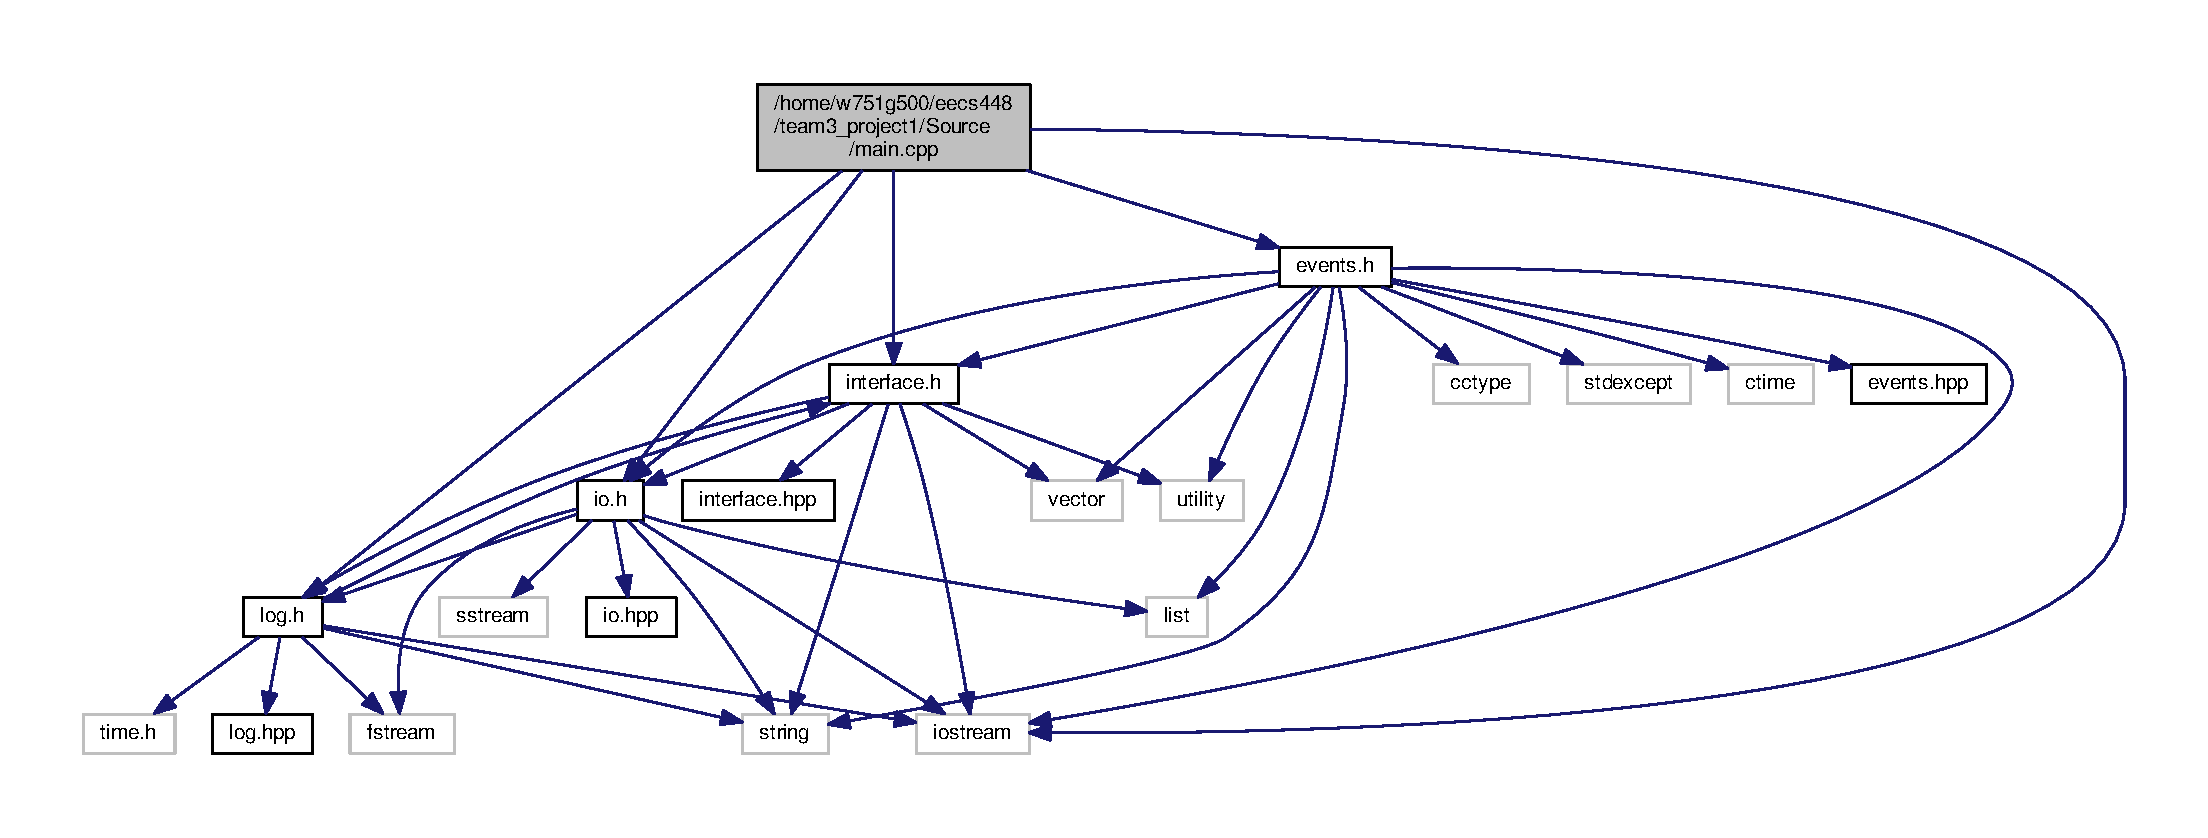
\includegraphics[width=350pt]{main_8cpp__incl}
\end{center}
\end{figure}
\subsection*{Functions}
\begin{DoxyCompactItemize}
\item 
int {\bfseries main} (int argc, char $\ast$$\ast$argv)\hypertarget{main_8cpp_a3c04138a5bfe5d72780bb7e82a18e627}{}\label{main_8cpp_a3c04138a5bfe5d72780bb7e82a18e627}

\end{DoxyCompactItemize}


\subsection{Detailed Description}
driver for project 

\begin{DoxyAuthor}{Author}
Team 3 
\end{DoxyAuthor}
\begin{DoxyDate}{Date}

\end{DoxyDate}

%--- End generated contents ---

% Index
\backmatter
\newpage
\phantomsection
\clearemptydoublepage
\addcontentsline{toc}{chapter}{Index}
\printindex

\end{document}
